\chapter{Análisis amortizado}

\index{análisis amortizado}

La complejidad temporal de un algoritmo
a menudo es fácil de analizar
simplemente examinando la estructura
del algoritmo:
qué bucles contiene el algoritmo
y cuántas veces se ejecutan los bucles.
Sin embargo, a veces un análisis directo
no da una imagen real de la eficiencia del algoritmo.

\key{Análisis amortizado} se puede utilizar para analizar
algoritmos que contienen operaciones cuya
complejidad temporal varía.
La idea es estimar el tiempo total utilizado para
todas esas operaciones durante la
ejecución del algoritmo, en lugar de centrarse
en operaciones individuales.

\section{Método de dos punteros}

\index{método de dos punteros}

En el \key{método de dos punteros},
se utilizan dos punteros para
iterar a través de los valores de la matriz.
Ambos punteros pueden moverse solo en una dirección,
lo que garantiza que el algoritmo funcione de manera eficiente.
A continuación, analizaremos dos problemas que se pueden resolver
utilizando el método de dos punteros.

\subsubsection{Suma de subarreglos}

Como primer ejemplo,
considere un problema en el que se nos
da un arreglo de $n$ enteros positivos
y una suma objetivo $x$,
y queremos encontrar un subarreglo cuya suma sea $x$
o informar que no existe tal subarreglo.

Por ejemplo, el arreglo
\begin{center}
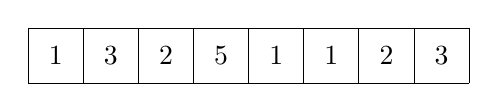
\begin{tikzpicture}[scale=0.7]
\draw (0,0) grid (8,1);

\node at (0.5,0.5) {$1$};
\node at (1.5,0.5) {$3$};
\node at (2.5,0.5) {$2$};
\node at (3.5,0.5) {$5$};
\node at (4.5,0.5) {$1$};
\node at (5.5,0.5) {$1$};
\node at (6.5,0.5) {$2$};
\node at (7.5,0.5) {$3$};
\end{tikzpicture}
\end{center}
contiene un subarreglo cuya suma es 8:
\begin{center}
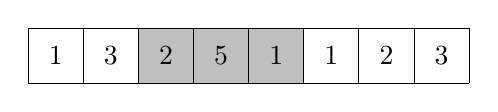
\begin{tikzpicture}[scale=0.7]
\fill[color=lightgray] (2,0) rectangle (5,1);
\draw (0,0) grid (8,1);

\node at (0.5,0.5) {$1$};
\node at (1.5,0.5) {$3$};
\node at (2.5,0.5) {$2$};
\node at (3.5,0.5) {$5$};
\node at (4.5,0.5) {$1$};
\node at (5.5,0.5) {$1$};
\node at (6.5,0.5) {$2$};
\node at (7.5,0.5) {$3$};
\end{tikzpicture}
\end{center}

Este problema se puede resolver en
tiempo $O(n)$ utilizando el método de dos punteros.
La idea es mantener punteros que apunten al
primer y último valor de un subarreglo.
En cada turno, el puntero izquierdo se mueve un paso
hacia la derecha, y el puntero derecho se mueve hacia la derecha
siempre que la suma del subarreglo resultante sea como máximo $x$.
Si la suma se convierte exactamente en $x$,
se ha encontrado una solución.

Como ejemplo, considere el siguiente arreglo
y una suma objetivo $x=8$:
\begin{center}
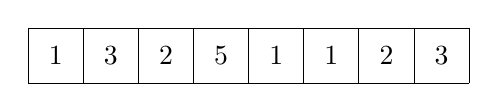
\begin{tikzpicture}[scale=0.7]
\draw (0,0) grid (8,1);

\node at (0.5,0.5) {$1$};
\node at (1.5,0.5) {$3$};
\node at (2.5,0.5) {$2$};
\node at (3.5,0.5) {$5$};
\node at (4.5,0.5) {$1$};
\node at (5.5,0.5) {$1$};
\node at (6.5,0.5) {$2$};
\node at (7.5,0.5) {$3$};
\end{tikzpicture}
\end{center}

El subarreglo inicial contiene los valores
1, 3 y 2 cuya suma es 6:

\begin{center}
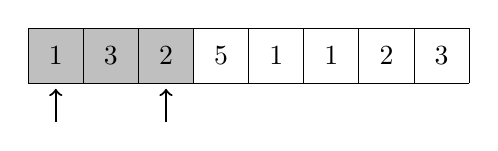
\begin{tikzpicture}[scale=0.7]
\fill[color=lightgray] (0,0) rectangle (3,1);
\draw (0,0) grid (8,1);

\node at (0.5,0.5) {$1$};
\node at (1.5,0.5) {$3$};
\node at (2.5,0.5) {$2$};
\node at (3.5,0.5) {$5$};
\node at (4.5,0.5) {$1$};
\node at (5.5,0.5) {$1$};
\node at (6.5,0.5) {$2$};
\node at (7.5,0.5) {$3$};

\draw[thick,->] (0.5,-0.7) -- (0.5,-0.1);
\draw[thick,->] (2.5,-0.7) -- (2.5,-0.1);
\end{tikzpicture}
\end{center}

Luego, el puntero izquierdo se mueve un paso hacia la derecha.
El puntero derecho no se mueve, porque de lo contrario
la suma del subarreglo excedería $x$.

\begin{center}
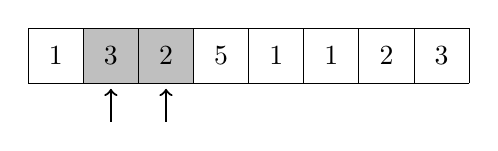
\begin{tikzpicture}[scale=0.7]
\fill[color=lightgray] (1,0) rectangle (3,1);
\draw (0,0) grid (8,1);

\node at (0.5,0.5) {$1$};
\node at (1.5,0.5) {$3$};
\node at (2.5,0.5) {$2$};
\node at (3.5,0.5) {$5$};
\node at (4.5,0.5) {$1$};
\node at (5.5,0.5) {$1$};
\node at (6.5,0.5) {$2$};
\node at (7.5,0.5) {$3$};

\draw[thick,->] (1.5,-0.7) -- (1.5,-0.1);
\draw[thick,->] (2.5,-0.7) -- (2.5,-0.1);
\end{tikzpicture}
\end{center}

Nuevamente, el puntero izquierdo se mueve un paso hacia la derecha,
y esta vez el puntero derecho se mueve tres
pasos hacia la derecha.
La suma del subarreglo es $2+5+1=8$, por lo que se ha encontrado un subarreglo
cuya suma es $x$.

\begin{center}
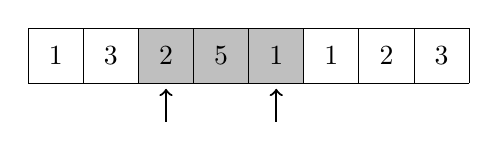
\begin{tikzpicture}[scale=0.7]
\fill[color=lightgray] (2,0) rectangle (5,1);
\draw (0,0) grid (8,1);

\node at (0.5,0.5) {$1$};
\node at (1.5,0.5) {$3$};
\node at (2.5,0.5) {$2$};
\node at (3.5,0.5) {$5$};
\node at (4.5,0.5) {$1$};
\node at (5.5,0.5) {$1$};
\node at (6.5,0.5) {$2$};
\node at (7.5,0.5) {$3$};

\draw[thick,->] (2.5,-0.7) -- (2.5,-0.1);
\draw[thick,->] (4.5,-0.7) -- (4.5,-0.1);
\end{tikzpicture}
\end{center}

El tiempo de ejecución del algoritmo depende de
la cantidad de pasos que se mueve el puntero derecho.
Si bien no existe un límite superior útil sobre cuántos pasos el
puntero puede moverse en un \emph{solo} turno.
sabemos que el puntero se mueve \emph{un total de}
$O(n)$ pasos durante el algoritmo,
porque solo se mueve hacia la derecha.

Dado que tanto el puntero izquierdo como el derecho
se mueven $O(n)$ pasos durante el algoritmo,
el algoritmo funciona en tiempo $O(n)$.

\subsubsection{Problema 2SUM}

\index{problema 2SUM}

Otro problema que se puede resolver utilizando
el método de los dos punteros es el siguiente problema,
también conocido como el problema de \key{2SUM}:
dada una matriz de $n$ números y
una suma objetivo $x$, encontrar
dos valores de la matriz tales que su suma sea $x$,
o informar que no existen tales valores.

Para resolver el problema, primero
ordenamos los valores de la matriz en orden creciente.
Después de eso, iteramos a través de la matriz usando
dos punteros.
El puntero izquierdo comienza en el primer valor
y se mueve un paso a la derecha en cada vuelta.
El puntero derecho comienza en el último valor
y siempre se mueve hacia la izquierda hasta que la suma de los
valores izquierdo y derecho es como máximo $x$.
Si la suma es exactamente $x$,
se ha encontrado una solución.

Por ejemplo, considere la siguiente matriz
y una suma objetivo $x=12$:
\begin{center}
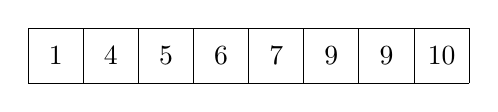
\begin{tikzpicture}[scale=0.7]
\draw (0,0) grid (8,1);

\node at (0.5,0.5) {$1$};
\node at (1.5,0.5) {$4$};
\node at (2.5,0.5) {$5$};
\node at (3.5,0.5) {$6$};
\node at (4.5,0.5) {$7$};
\node at (5.5,0.5) {$9$};
\node at (6.5,0.5) {$9$};
\node at (7.5,0.5) {$10$};
\end{tikzpicture}
\end{center}

Las posiciones iniciales de los punteros
son las siguientes.
La suma de los valores es $1+10=11$
que es menor que $x$.

\begin{center}
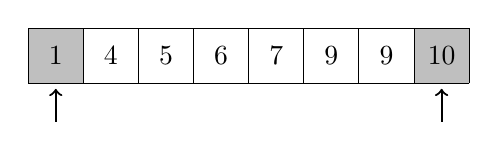
\begin{tikzpicture}[scale=0.7]
\fill[color=lightgray] (0,0) rectangle (1,1);
\fill[color=lightgray] (7,0) rectangle (8,1);
\draw (0,0) grid (8,1);

\node at (0.5,0.5) {$1$};
\node at (1.5,0.5) {$4$};
\node at (2.5,0.5) {$5$};
\node at (3.5,0.5) {$6$};
\node at (4.5,0.5) {$7$};
\node at (5.5,0.5) {$9$};
\node at (6.5,0.5) {$9$};
\node at (7.5,0.5) {$10$};

\draw[thick,->] (0.5,-0.7) -- (0.5,-0.1);
\draw[thick,->] (7.5,-0.7) -- (7.5,-0.1);
\end{tikzpicture}
\end{center}

Luego, el puntero izquierdo se mueve un paso a la derecha.
El puntero derecho se mueve tres pasos a la izquierda,
y la suma se convierte en $4+7=11$.

\begin{center}
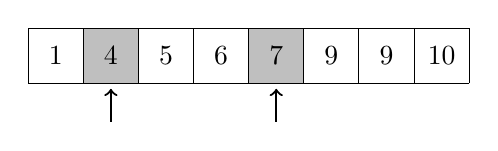
\begin{tikzpicture}[scale=0.7]
\fill[color=lightgray] (1,0) rectangle (2,1);
\fill[color=lightgray] (4,0) rectangle (5,1);
\draw (0,0) grid (8,1);

\node at (0.5,0.5) {$1$};
\node at (1.5,0.5) {$4$};
\node at (2.5,0.5) {$5$};
\node at (3.5,0.5) {$6$};
\node at (4.5,0.5) {$7$};
\node at (5.5,0.5) {$9$};
\node at (6.5,0.5) {$9$};
\node at (7.5,0.5) {$10$};

\draw[thick,->] (1.5,-0.7) -- (1.5,-0.1);
\draw[thick,->] (4.5,-0.7) -- (4.5,-0.1);
\end{tikzpicture}
\end{center}

Después de esto, el puntero izquierdo se mueve un paso a la derecha de nuevo.
El puntero derecho no se mueve, y una solución
$5+7=12$ ha sido encontrada.

\begin{center}
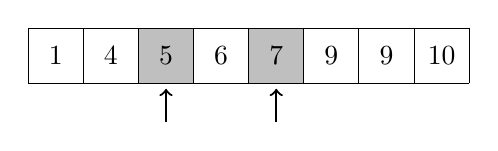
\begin{tikzpicture}[scale=0.7]
\fill[color=lightgray] (2,0) rectangle (3,1);
\fill[color=lightgray] (4,0) rectangle (5,1);
\draw (0,0) grid (8,1);

\node at (0.5,0.5) {$1$};
\node at (1.5,0.5) {$4$};
\node at (2.5,0.5) {$5$};
\node at (3.5,0.5) {$6$};
\node at (4.5,0.5) {$7$};
\node at (5.5,0.5) {$9$};
\node at (6.5,0.5) {$9$};
\node at (7.5,0.5) {$10$};

\draw[thick,->] (2.5,-0.7) -- (2.5,-0.1);
\draw[thick,->] (4.5,-0.7) -- (4.5,-0.1);
\end{tikzpicture}
\end{center}

El tiempo de ejecución del algoritmo es
$O(n \log n)$, porque primero ordena
la matriz en $O(n \log n)$ tiempo,
y luego ambos punteros se mueven $O(n)$ pasos.

Tenga en cuenta que es posible resolver el problema
de otra manera en $O(n \log n)$ tiempo usando la búsqueda binaria.
En tal solución, iteramos a través de la matriz
y para cada valor de la matriz, tratamos de encontrar otro
valor que produzca la suma $x$.
Esto se puede hacer realizando $n$ búsquedas binarias,
cada una de las cuales tarda $O(\log n)$ tiempo.

\index{3SUM problem}
Un problema más difícil es 
el problema de \key{3SUM} que pide
encontrar \emph{tres} valores de la matriz
cuya suma es $x$.
Utilizando la idea del algoritmo anterior,
este problema se puede resolver en $O(n^2)$ tiempo\footnote{Durante mucho tiempo,
se pensó que resolver
el problema de 3SUM más eficientemente que en $O(n^2)$ tiempo
no sería posible.
Sin embargo, en 2014, resultó \cite{gro14}
que este no es el caso.}.
¿Puedes ver cómo?

\section{Elementos más pequeños cercanos}

\index{nearest smaller elements}

El análisis amortizado se utiliza a menudo para
estimar el número de operaciones
realizadas en una estructura de datos.
Las operaciones pueden estar distribuidas de forma desigual, de modo que
la mayoría de las operaciones ocurren durante una
cierta fase del algoritmo, pero el total
número de operaciones es limitado.

Como ejemplo, considere el problema
de encontrar para cada elemento de la matriz
el \key{elemento más pequeño cercano}, es decir,
el primer elemento más pequeño que precede al elemento
en la matriz.
Es posible que no exista tal elemento,
en cuyo caso el algoritmo debe reportar esto.
A continuación veremos cómo el problema puede ser
resuelto eficientemente utilizando una estructura de pila.

Recorremos la matriz de izquierda a derecha
y mantenemos una pila de elementos de la matriz.
En cada posición de la matriz, eliminamos elementos de la pila
hasta que el elemento superior sea menor que el
elemento actual, o la pila esté vacía.
Luego, informamos que el elemento superior es
el elemento más pequeño cercano del elemento actual,
o si la pila está vacía, no existe tal elemento.
Finalmente, agregamos el elemento actual a la pila.
Como ejemplo, considere la siguiente matriz:
\begin{center}
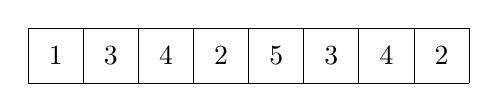
\begin{tikzpicture}[scale=0.7]
\draw (0,0) grid (8,1);

\node at (0.5,0.5) {$1$};
\node at (1.5,0.5) {$3$};
\node at (2.5,0.5) {$4$};
\node at (3.5,0.5) {$2$};
\node at (4.5,0.5) {$5$};
\node at (5.5,0.5) {$3$};
\node at (6.5,0.5) {$4$};
\node at (7.5,0.5) {$2$};
\end{tikzpicture}
\end{center}

Primero, los elementos 1, 3 y 4 se agregan a la pila,
porque cada elemento es mayor que el elemento anterior.
Por lo tanto, el elemento más pequeño cercano de 4 es 3,
y el elemento más pequeño cercano de 3 es 1.
\begin{center}
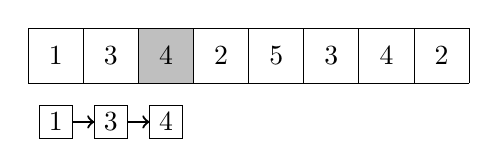
\begin{tikzpicture}[scale=0.7]
\fill[color=lightgray] (2,0) rectangle (3,1);
\draw (0,0) grid (8,1);

\node at (0.5,0.5) {$1$};
\node at (1.5,0.5) {$3$};
\node at (2.5,0.5) {$4$};
\node at (3.5,0.5) {$2$};
\node at (4.5,0.5) {$5$};
\node at (5.5,0.5) {$3$};
\node at (6.5,0.5) {$4$};
\node at (7.5,0.5) {$2$};

\draw (0.2,0.2-1.2) rectangle (0.8,0.8-1.2);
\draw (1.2,0.2-1.2) rectangle (1.8,0.8-1.2);
\draw (2.2,0.2-1.2) rectangle (2.8,0.8-1.2);

\node at (0.5,0.5-1.2) {$1$};
\node at (1.5,0.5-1.2) {$3$};
\node at (2.5,0.5-1.2) {$4$};

\draw[->,thick] (0.8,0.5-1.2) -- (1.2,0.5-1.2);
\draw[->,thick] (1.8,0.5-1.2) -- (2.2,0.5-1.2);
\end{tikzpicture}
\end{center}

El siguiente elemento 2 es menor que los dos elementos superiores
en la pila.
Por lo tanto, los elementos 3 y 4 se eliminan de la pila,
y luego el elemento 2 se agrega a la pila.
Su elemento más pequeño cercano es 1:
\begin{center}
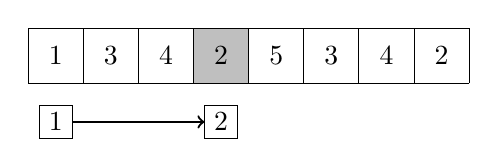
\begin{tikzpicture}[scale=0.7]
\fill[color=lightgray] (3,0) rectangle (4,1);
\draw (0,0) grid (8,1);

\node at (0.5,0.5) {$1$};
\node at (1.5,0.5) {$3$};
\node at (2.5,0.5) {$4$};
\node at (3.5,0.5) {$2$};
\node at (4.5,0.5) {$5$};
\node at (5.5,0.5) {$3$};
\node at (6.5,0.5) {$4$};
\node at (7.5,0.5) {$2$};

\draw (0.2,0.2-1.2) rectangle (0.8,0.8-1.2);
\draw (3.2,0.2-1.2) rectangle (3.8,0.8-1.2);

\node at (0.5,0.5-1.2) {$1$};
\node at (3.5,0.5-1.2) {$2$};

\draw[->,thick] (0.8,0.5-1.2) -- (3.2,0.5-1.2);
\end{tikzpicture}
\end{center}

Luego, el elemento 5 es mayor que el elemento 2,
por lo que se agregará a la pila, y
su elemento más pequeño cercano es 2:
\begin{center}
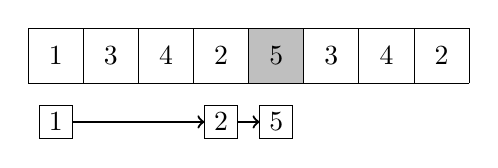
\begin{tikzpicture}[scale=0.7]
\fill[color=lightgray] (4,0) rectangle (5,1);
\draw (0,0) grid (8,1);

\node at (0.5,0.5) {$1$};
\node at (1.5,0.5) {$3$};
\node at (2.5,0.5) {$4$};
\node at (3.5,0.5) {$2$};
\node at (4.5,0.5) {$5$};
\node at (5.5,0.5) {$3$};
\node at (6.5,0.5) {$4$};
\node at (7.5,0.5) {$2$};

\draw (0.2,0.2-1.2) rectangle (0.8,0.8-1.2);
\draw (3.2,0.2-1.2) rectangle (3.8,0.8-1.2);
\draw (4.2,0.2-1.2) rectangle (4.8,0.8-1.2);

\node at (0.5,0.5-1.2) {$1$};
\node at (3.5,0.5-1.2) {$2$};
\node at (4.5,0.5-1.2) {$5$};

\draw[->,thick] (0.8,0.5-1.2) -- (3.2,0.5-1.2);
\draw[->,thick] (3.8,0.5-1.2) -- (4.2,0.5-1.2);
\end{tikzpicture}
\end{center}

Después de esto, el elemento 5 se elimina de la pila
y los elementos 3 y 4 se agregan a la pila:
\begin{center}
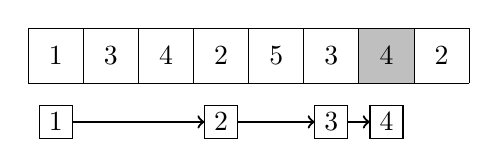
\begin{tikzpicture}[scale=0.7]
\fill[color=lightgray] (6,0) rectangle (7,1);
\draw (0,0) grid (8,1);

\node at (0.5,0.5) {$1$};
\node at (1.5,0.5) {$3$};
\node at (2.5,0.5) {$4$};
\node at (3.5,0.5) {$2$};
\node at (4.5,0.5) {$5$};
\node at (5.5,0.5) {$3$};
\node at (6.5,0.5) {$4$};
\node at (7.5,0.5) {$2$};

\draw (0.2,0.2-1.2) rectangle (0.8,0.8-1.2);
\draw (3.2,0.2-1.2) rectangle (3.8,0.8-1.2);
\draw (5.2,0.2-1.2) rectangle (5.8,0.8-1.2);
\draw (6.2,0.2-1.2) rectangle (6.8,0.8-1.2);

\node at (0.5,0.5-1.2) {$1$};
\node at (3.5,0.5-1.2) {$2$};
\node at (5.5,0.5-1.2) {$3$};
\node at (6.5,0.5-1.2) {$4$};

\draw[->,thick] (0.8,0.5-1.2) -- (3.2,0.5-1.2);
\draw[->,thick] (3.8,0.5-1.2) -- (5.2,0.5-1.2);
\draw[->,thick] (5.8,0.5-1.2) -- (6.2,0.5-1.2);
\end{tikzpicture}
\end{center}

Finalmente, todos los elementos excepto 1 se eliminan
de la pila y el último elemento 2
se agrega a la pila:

\begin{center}
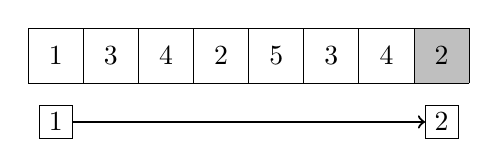
\begin{tikzpicture}[scale=0.7]
\fill[color=lightgray] (7,0) rectangle (8,1);
\draw (0,0) grid (8,1);

\node at (0.5,0.5) {$1$};
\node at (1.5,0.5) {$3$};
\node at (2.5,0.5) {$4$};
\node at (3.5,0.5) {$2$};
\node at (4.5,0.5) {$5$};
\node at (5.5,0.5) {$3$};
\node at (6.5,0.5) {$4$};
\node at (7.5,0.5) {$2$};

\draw (0.2,0.2-1.2) rectangle (0.8,0.8-1.2);
\draw (7.2,0.2-1.2) rectangle (7.8,0.8-1.2);

\node at (0.5,0.5-1.2) {$1$};
\node at (7.5,0.5-1.2) {$2$};

\draw[->,thick] (0.8,0.5-1.2) -- (7.2,0.5-1.2);
\end{tikzpicture}
\end{center}

La eficiencia del algoritmo depende de
la cantidad total de operaciones de pila.
Si el elemento actual es mayor que
el elemento superior en la pila, se agrega directamente
a la pila, lo cual es eficiente.
Sin embargo, a veces la pila puede contener varios
elementos más grandes y lleva tiempo eliminarlos.
Aún así, cada elemento se agrega \emph{exactamente una vez} a la pila
y se elimina \emph{como máximo una vez} de la pila.
Por lo tanto, cada elemento provoca $O(1)$ operaciones de pila,
y el algoritmo funciona en tiempo $O(n)$.

\section{Mínimo de ventana deslizante}

\index{ventana deslizante}
\index{mínimo de ventana deslizante}


Una \key{ventana deslizante} es una submatriz de tamaño constante
que se mueve de izquierda a derecha a través de la matriz.
En cada posición de la ventana,
queremos calcular alguna información
sobre los elementos dentro de la ventana.
En esta sección, nos centramos en el problema
de mantener el \key{mínimo de la ventana deslizante},
lo que significa que
deberíamos reportar el valor más pequeño dentro de cada ventana.

El mínimo de la ventana deslizante se puede calcular
usando una idea similar a la que usamos para calcular
los elementos más cercanos más pequeños.
Mantenemos una cola
donde cada elemento es más grande que
el elemento anterior,
y el primer elemento
siempre corresponde al elemento mínimo dentro de la ventana.
Después de cada movimiento de la ventana,
eliminamos elementos del final de la cola
hasta que el último elemento de la cola
sea más pequeño que el nuevo elemento de la ventana,
o la cola se vacíe.
También eliminamos el primer elemento de la cola
si ya no está dentro de la ventana.
Finalmente, añadimos el nuevo elemento de la ventana
al final de la cola.

Como ejemplo, considere la siguiente matriz:

\begin{center}
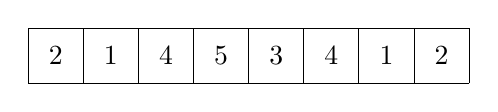
\begin{tikzpicture}[scale=0.7]
\draw (0,0) grid (8,1);

\node at (0.5,0.5) {$2$};
\node at (1.5,0.5) {$1$};
\node at (2.5,0.5) {$4$};
\node at (3.5,0.5) {$5$};
\node at (4.5,0.5) {$3$};
\node at (5.5,0.5) {$4$};
\node at (6.5,0.5) {$1$};
\node at (7.5,0.5) {$2$};
\end{tikzpicture}
\end{center}

Supongamos que el tamaño de la ventana deslizante es 4.
En la primera posición de la ventana, el valor más pequeño es 1:
\begin{center}
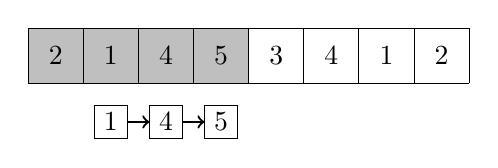
\begin{tikzpicture}[scale=0.7]
\fill[color=lightgray] (0,0) rectangle (4,1);
\draw (0,0) grid (8,1);

\node at (0.5,0.5) {$2$};
\node at (1.5,0.5) {$1$};
\node at (2.5,0.5) {$4$};
\node at (3.5,0.5) {$5$};
\node at (4.5,0.5) {$3$};
\node at (5.5,0.5) {$4$};
\node at (6.5,0.5) {$1$};
\node at (7.5,0.5) {$2$};

\draw (1.2,0.2-1.2) rectangle (1.8,0.8-1.2);
\draw (2.2,0.2-1.2) rectangle (2.8,0.8-1.2);
\draw (3.2,0.2-1.2) rectangle (3.8,0.8-1.2);

\node at (1.5,0.5-1.2) {$1$};
\node at (2.5,0.5-1.2) {$4$};
\node at (3.5,0.5-1.2) {$5$};

\draw[->,thick] (1.8,0.5-1.2) -- (2.2,0.5-1.2);
\draw[->,thick] (2.8,0.5-1.2) -- (3.2,0.5-1.2);
\end{tikzpicture}
\end{center}

Luego la ventana se mueve un paso a la derecha.
El nuevo elemento 3 es más pequeño que los elementos
4 y 5 en la cola, por lo que los elementos 4 y 5
se eliminan de la cola
y el elemento 3 se añade a la cola.
El valor más pequeño sigue siendo 1.
\begin{center}
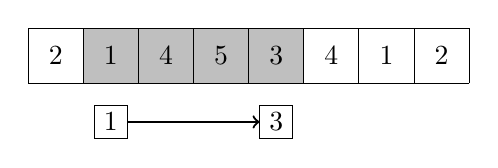
\begin{tikzpicture}[scale=0.7]
\fill[color=lightgray] (1,0) rectangle (5,1);
\draw (0,0) grid (8,1);

\node at (0.5,0.5) {$2$};
\node at (1.5,0.5) {$1$};
\node at (2.5,0.5) {$4$};
\node at (3.5,0.5) {$5$};
\node at (4.5,0.5) {$3$};
\node at (5.5,0.5) {$4$};
\node at (6.5,0.5) {$1$};
\node at (7.5,0.5) {$2$};

\draw (1.2,0.2-1.2) rectangle (1.8,0.8-1.2);
\draw (4.2,0.2-1.2) rectangle (4.8,0.8-1.2);

\node at (1.5,0.5-1.2) {$1$};
\node at (4.5,0.5-1.2) {$3$};

\draw[->,thick] (1.8,0.5-1.2) -- (4.2,0.5-1.2);
\end{tikzpicture}
\end{center}

Después de esto, la ventana se mueve de nuevo,
y el elemento más pequeño 1
ya no pertenece a la ventana.
Por lo tanto, se elimina de la cola y el más pequeño
el valor ahora es 3. También el nuevo elemento 4
se añade a la cola.
\begin{center}
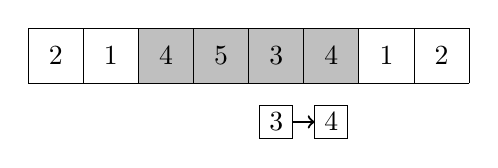
\begin{tikzpicture}[scale=0.7]
\fill[color=lightgray] (2,0) rectangle (6,1);
\draw (0,0) grid (8,1);

\node at (0.5,0.5) {$2$};
\node at (1.5,0.5) {$1$};
\node at (2.5,0.5) {$4$};
\node at (3.5,0.5) {$5$};
\node at (4.5,0.5) {$3$};
\node at (5.5,0.5) {$4$};
\node at (6.5,0.5) {$1$};
\node at (7.5,0.5) {$2$};

\draw (4.2,0.2-1.2) rectangle (4.8,0.8-1.2);
\draw (5.2,0.2-1.2) rectangle (5.8,0.8-1.2);

\node at (4.5,0.5-1.2) {$3$};
\node at (5.5,0.5-1.2) {$4$};

\draw[->,thick] (4.8,0.5-1.2) -- (5.2,0.5-1.2);
\end{tikzpicture}
\end{center}

El siguiente nuevo elemento 1 es más pequeño que todos los elementos
en la cola.
Por lo tanto, todos los elementos se eliminan de la cola
y solo contendrá el elemento 1:
\begin{center}
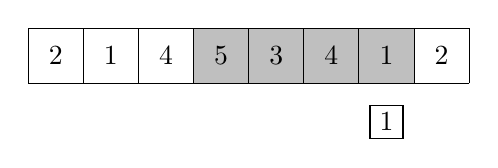
\begin{tikzpicture}[scale=0.7]
\fill[color=lightgray] (3,0) rectangle (7,1);
\draw (0,0) grid (8,1);

\node at (0.5,0.5) {$2$};
\node at (1.5,0.5) {$1$};
\node at (2.5,0.5) {$4$};
\node at (3.5,0.5) {$5$};
\node at (4.5,0.5) {$3$};
\node at (5.5,0.5) {$4$};
\node at (6.5,0.5) {$1$};
\node at (7.5,0.5) {$2$};

\draw (6.2,0.2-1.2) rectangle (6.8,0.8-1.2);

\node at (6.5,0.5-1.2) {$1$};
\end{tikzpicture}
\end{center}

Finalmente la ventana alcanza su última posición.
El elemento 2 se añade a la cola,
pero el valor más pequeño dentro de la ventana
sigue siendo 1.
\begin{center}
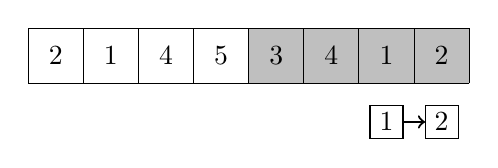
\begin{tikzpicture}[scale=0.7]
\fill[color=lightgray] (4,0) rectangle (8,1);
\draw (0,0) grid (8,1);

\node at (0.5,0.5) {$2$};
\node at (1.5,0.5) {$1$};
\node at (2.5,0.5) {$4$};
\node at (3.5,0.5) {$5$};
\node at (4.5,0.5) {$3$};
\node at (5.5,0.5) {$4$};
\node at (6.5,0.5) {$1$};
\node at (7.5,0.5) {$2$};

\draw (6.2,0.2-1.2) rectangle (6.8,0.8-1.2);
\draw (7.2,0.2-1.2) rectangle (7.8,0.8-1.2);

\node at (6.5,0.5-1.2) {$1$};
\node at (7.5,0.5-1.2) {$2$};

\draw[->,thick] (6.8,0.5-1.2) -- (7.2,0.5-1.2);
\end{tikzpicture}
\end{center}
Dado que cada elemento del arreglo
se agrega a la cola exactamente una vez y
se elimina de la cola como máximo una vez,
el algoritmo funciona en tiempo $O(n)$. 
